\documentclass[11pt]{article}
\usepackage[margin=1in]{geometry}

\usepackage{tikz}
\begin{document}


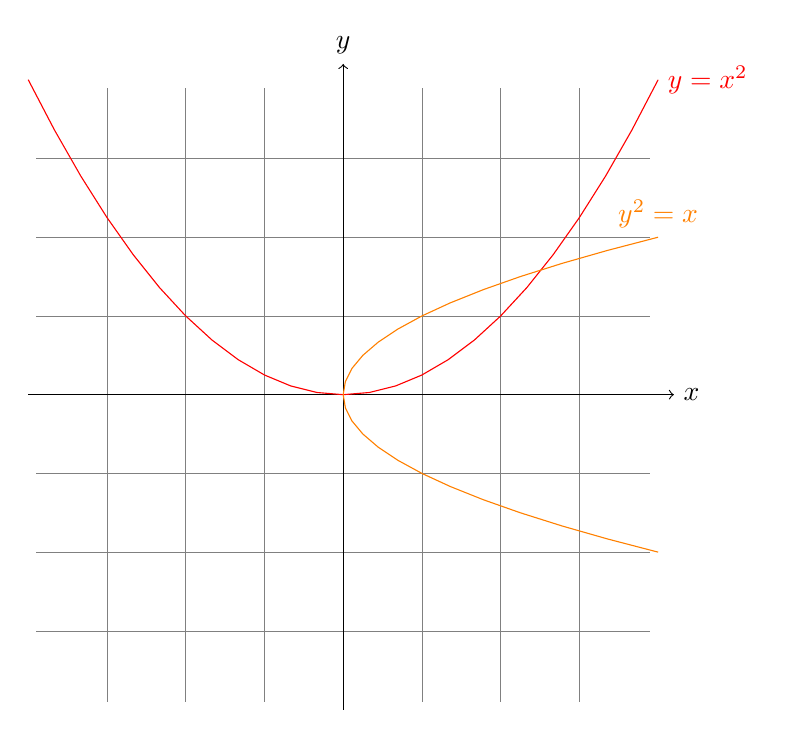
\begin{tikzpicture}
    \draw[very thin,color=gray] (-3.9,-3.9) grid (3.9, 3.9);
  
    \draw[->] (-4,0) -- (4.2,0) node[right] {$x$};
    \draw[->] (0,-4) -- (0,4.2) node[above] {$y$};

    \draw[color=red, domain=-2:2] plot (2*\x,{(\x)^2}) node[right] {$y = x^2$};
    \draw[color=orange, domain=-2:2] plot ({(\x)^2},\x) node[above] {$y^2 = x$};
    


\end{tikzpicture}
\\
\begin{tikzpicture}[transform shape,scale=0.2]
	\draw[color=red, domain=-3:9] plot ({4*((\x)+2)},{((\x )-3)^2}) node[right] {$y = x^2$};
	\end{tikzpicture}
\\
\begin{tikzpicture}[transform shape,scale=0.2]
	\draw[color=red, domain=-3:9] plot ({4*((\x)+2)},{((\x )-3)^2}) node[right] {$y = x^2$};
\end{tikzpicture}
\\
\begin{tikzpicture}[transform shape,scale=0.2]
	\draw[color=red, domain=-5:7] plot ({((\x )-1)^2},{4*((\x)-2)}) node[right] {$y = x^2$};
\end{tikzpicture}
\\
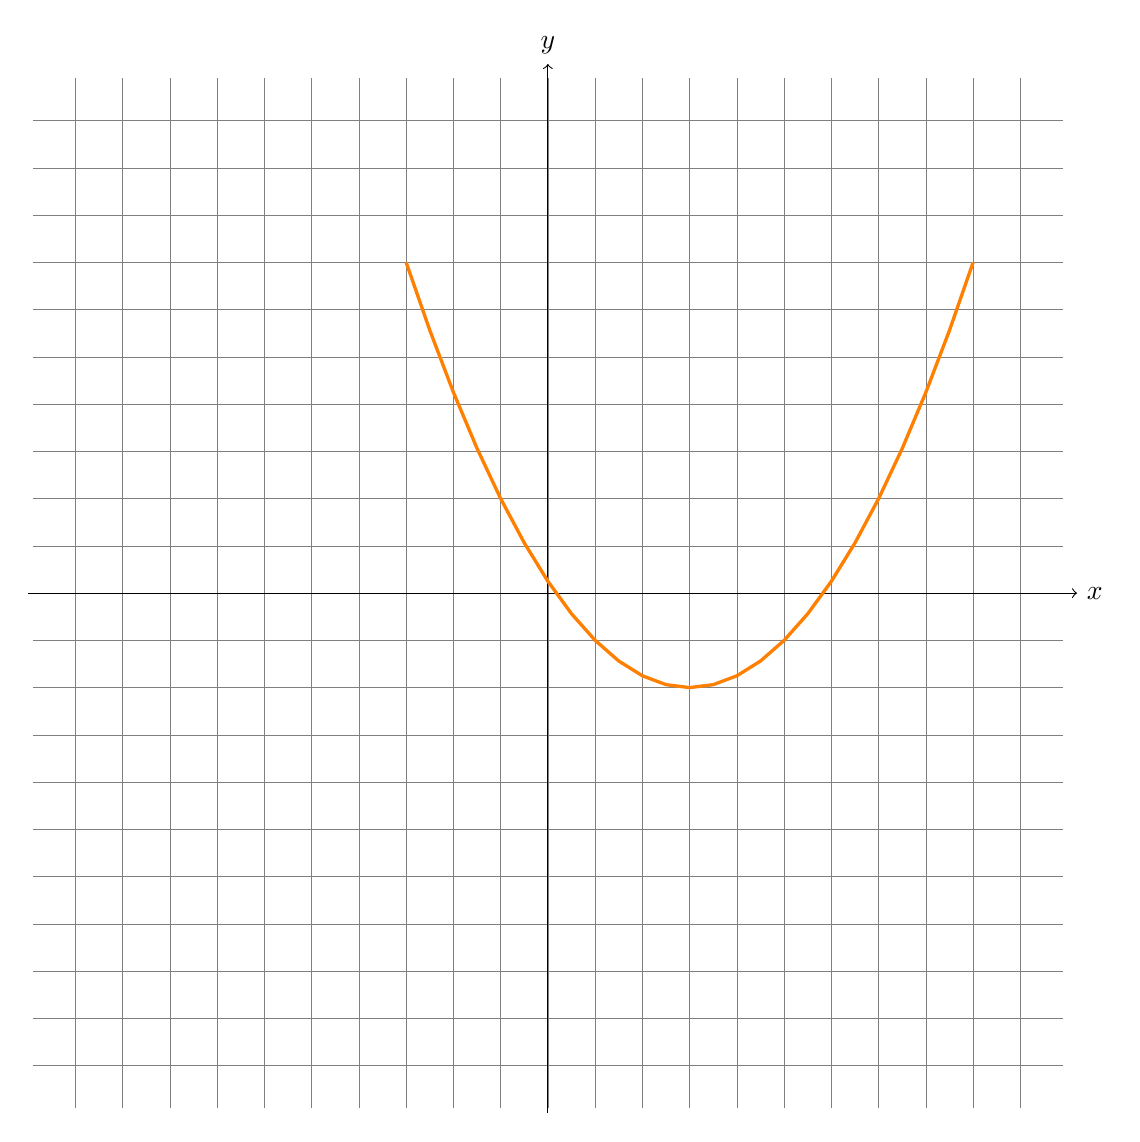
\begin{tikzpicture}[scale=0.6]
	\draw[very thin,color=gray] (-10.9,-10.9) grid (10.9, 10.9);
	\draw[->] (-11,0) -- (11.2,0) node[right] {$x$};
	\draw[->] (0,-11) -- (0,11.2) node[above] {$y$};
	\draw[color=orange,very thick, domain=-3:9] plot ({\x},{(\x - 3)^2 / 4 - 2}) node[right] {};
	
\end{tikzpicture}
\\
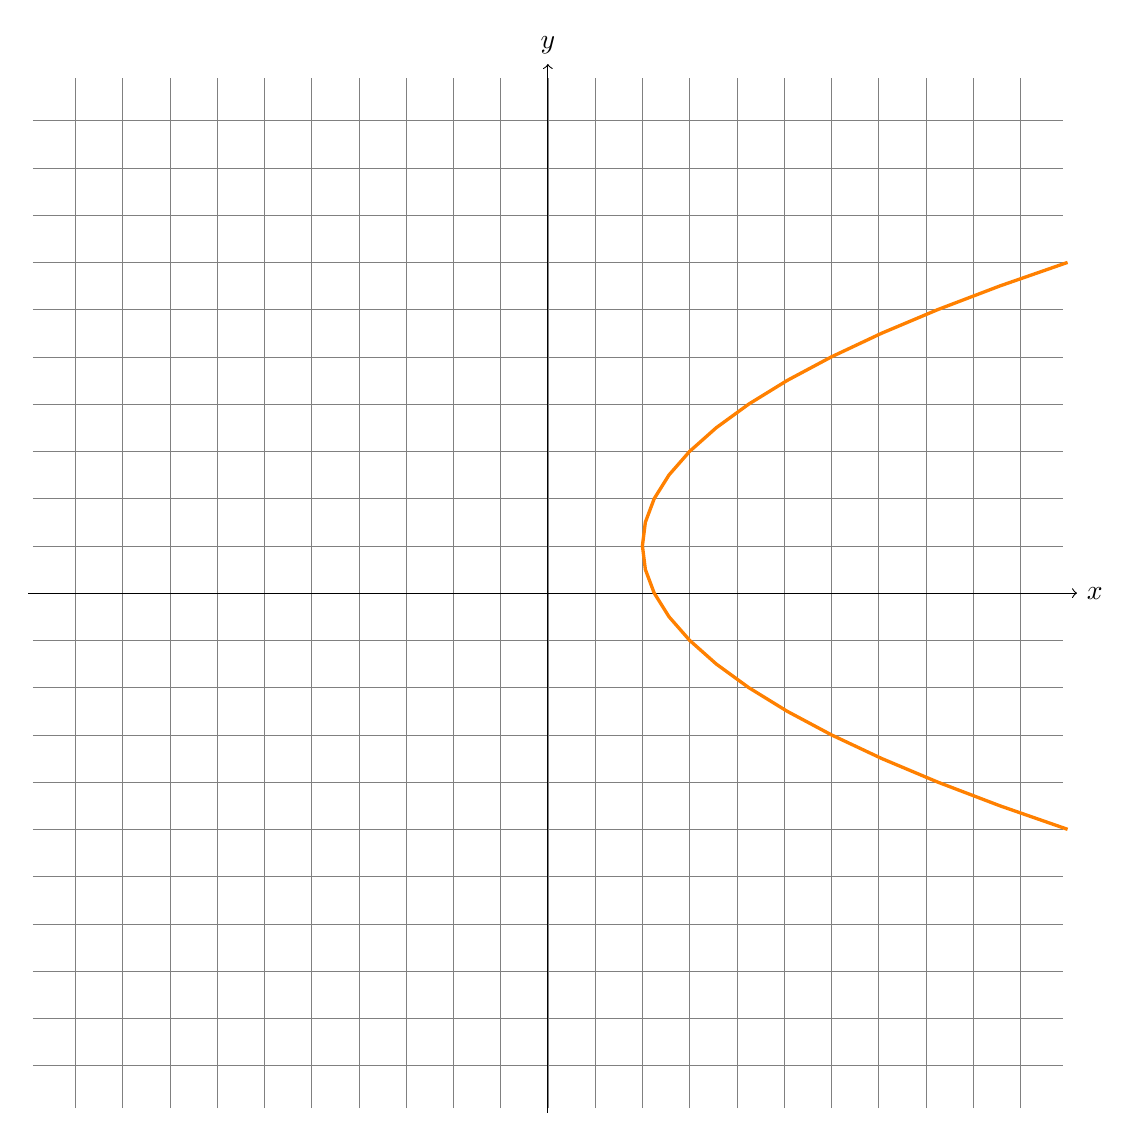
\begin{tikzpicture}[scale=0.6]
	\draw[very thin,color=gray] (-10.9,-10.9) grid (10.9, 10.9);
	\draw[->] (-11,0) -- (11.2,0) node[right] {$x$};
	\draw[->] (0,-11) -- (0,11.2) node[above] {$y$};
	\draw[color=orange,very thick, domain=-5:7] plot ({(\x - 1)^2 / 4 + 2},{\x}) node[right] {};
	
\end{tikzpicture}
\\
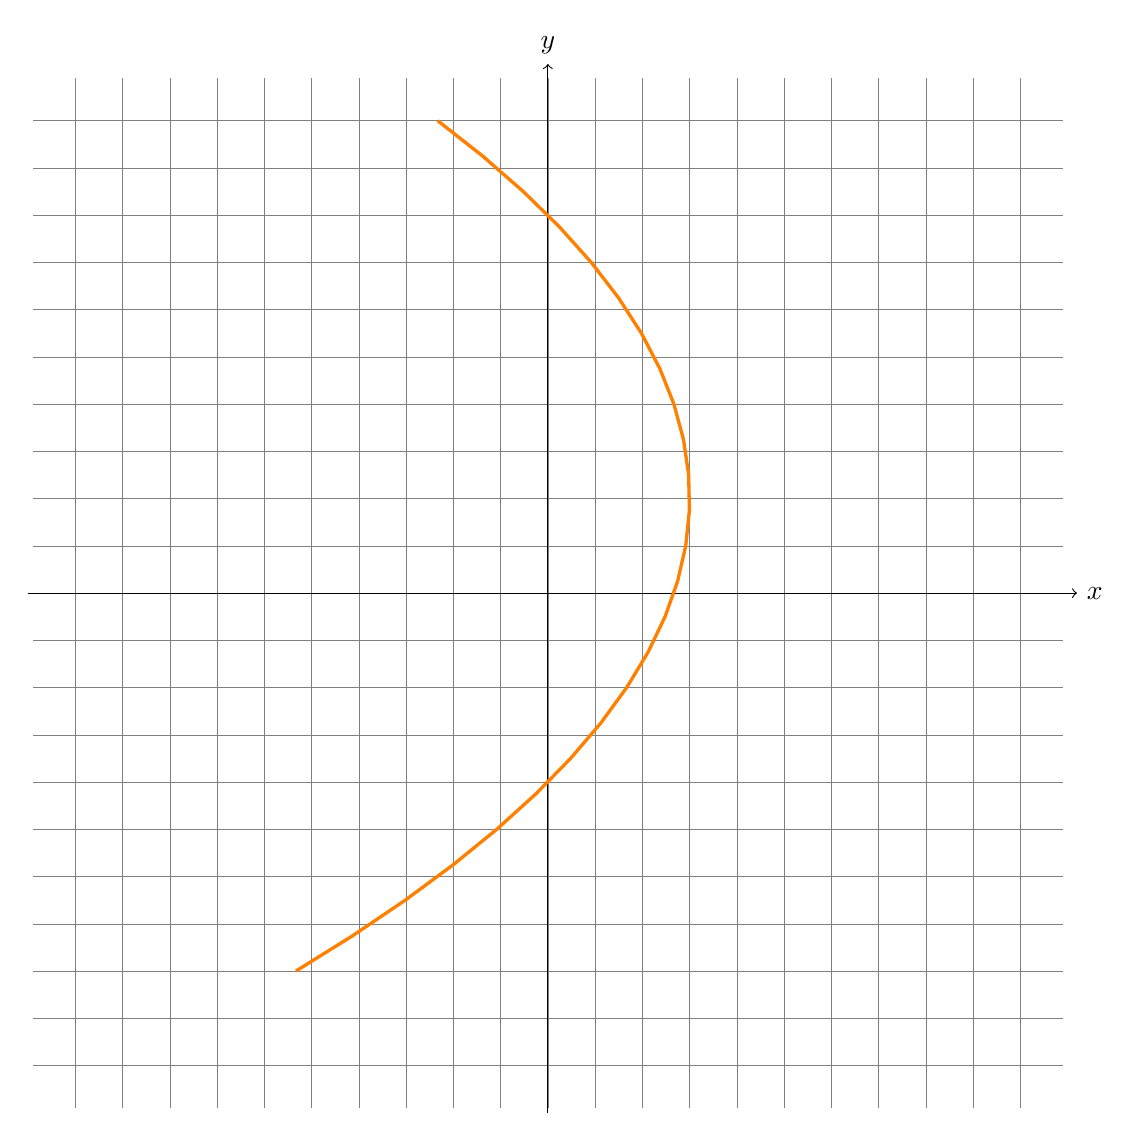
\begin{tikzpicture}[scale=0.6]
	\draw[very thin,color=gray] (-10.9,-10.9) grid (10.9, 10.9);
	\draw[->] (-11,0) -- (11.2,0) node[right] {$x$};
	\draw[->] (0,-11) -- (0,11.2) node[above] {$y$};
	\draw[color=orange,very thick, domain=-8:10] plot ({-(\x - 2)^2 / 12 + 3},{\x}) node[right] {};
	
\end{tikzpicture}
\end{document}
